
Feature analysis:

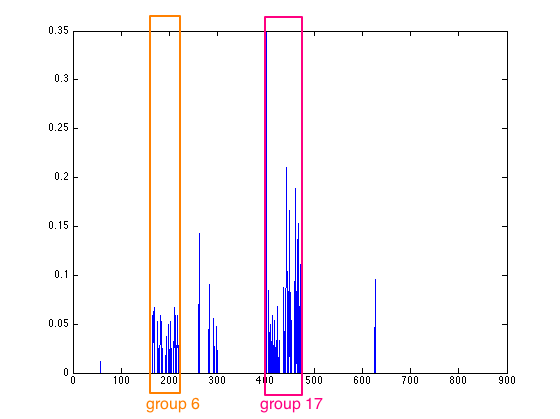
\includegraphics[width=0.18 \linewidth]{./images/mfcc_180.png}
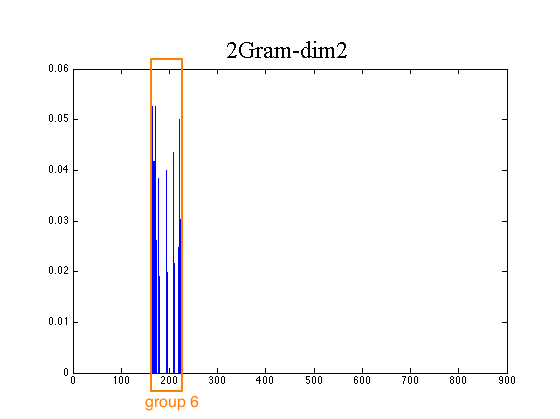
\includegraphics[width=0.20 \linewidth]{./images/ngram_202.png}

\footnotesize
\begin{tabular}{cccc}
\multicolumn{1}{c}{\bf Classifier }&\multicolumn{1}{c}{\bf Accuracy}  &\multicolumn{1}{c}{\bf Features} &\multicolumn{1}{c}{\bf Settings}
\\ \hline \\
linear SVM		&67.7273 		&MFCC 		&  \\
			& 70.4545  	& clean MFCC 	&  \\
poly SVM		&69.0909		&MFCC 		&  \\
			& 70.4545  	& clean MFCC 	& degree: 1  \\
			& 70 			& clean MFCC 	& degree: 2  \\
			& 70.4545  	& clean MFCC 	& degree: 3  \\
rbf SVM       	&70 			&MFCC 		&  \\
                     	&68  			&  MFCC (log) 	&  \\
          		&70.4545  		&  clean MFCC 	&  \\
          		&76.8182  		&  clean MFCC 	&  $\gamma = 7.9433$ \\
          		&{\bf 78.1818}  	&  clean MFCC + 2gram 	&    \\
sigmoid SVM     	&70.9091		&MFCC 		&  \\
       			&70.4545  		& clean MFCC 	&  \\
random forest    	&57			& clean MFCC	& 100 trees; 5 splits \\
       			&63  			& clean MFCC 	& 100 trees; 2 splits \\

\end{tabular}


